%- HandOut Flag -----------------------------------------------------------------------------------------
\makeatletter
\@ifundefined{ifHandout}{%
  \expandafter\newif\csname ifHandout\endcsname
}{}
\makeatother

%- D0cum3nt ----------------------------------------------------------------------------------------------
\documentclass[beamer,10pt]{standalone}   
%\documentclass[beamer,10pt,handout]{standalone}  \Handouttrue  

\ifHandout
	\setbeameroption{show notes} %print notes   
\fi

	
%- Packages ----------------------------------------------------------------------------------------------
\usepackage{custom-style}
\usepackage{math}




%--Beamer Style-----------------------------------------------------------------------------------------------
\usetheme{toninus}
\usepackage{animate}
\usetikzlibrary{positioning, arrows}
\usetikzlibrary{shapes}


%- Bibliography (Biber) ----------------------------------------------------------------------------------
\usepackage[backend=biber,style=alphabetic,maxnames=2]{biblatex}
\bibliography{bibfile.bib}

%===========================================================%
\begin{document}
%===========================================================%

%----------------------------------------------------+
\begin{frame}[fragile]{Keywords}
\tikzstyle{every picture}+=[remember picture]
	\begin{columns}
    	\begin{column}{.45\textwidth}
    		\onslide<5->{
			\tikz[baseline]{
		            \node[draw=orange!40,anchor=base,text width=5cm] (s1)
		            {The procedure to reduce the dimensions of a Phase Space (or the space of obsevables) in presence of constraints or symmetries.};
			}
		}
	\end{column}
    	\begin{column}{.45\textwidth}
    		\onslide<4->{
			 \tikz[baseline]{
		            \node[draw=blue!40,anchor=base, text width=5cm] (s2)
		            {Higher analogue of DGLie algebras where Jacobi holds up to homotopies.};
			}
		}
	\end{column}
	\end{columns}

	\vfill

	\begin{center}
		\large
		Construction and 
		\tikz[baseline]{
		            \node[fill=orange!20,anchor=base] (t1)
		            {Reduction};
			}
		of the 
		\tikz[baseline]{
	            \node[fill=blue!20,anchor=base] (t2)
	            {$L_\infty$-Algebra};
		} 
		\\ of \\
		\tikz[baseline]{
	            \node[fill=green!20,anchor=base] (t3)
	            {Observables};
		}
		associated with a
		\tikz[baseline]{
		            \node[fill=red!20,anchor=base] (t4)
		            {BV-module};
		}		
	\end{center}

	\vfill

	\begin{columns}
    	\begin{column}{.45\textwidth}
    		\onslide<3->{
	 		 \tikz[baseline]{
	            \node[draw=green!40,anchor=base,text width=5cm] (s3)
	            {Algebraic object encoding measurable quantities of a mechanical system.};
	         }
		}		   	
		\end{column}
    	\begin{column}{.45\textwidth}
    		\onslide<2->{
				\tikz[baseline]{
	            \node[draw=red!40,anchor=base,text width=5cm] (s4)
	            {Algebraic object encoding Cartan Calculus.};
	           }	
			}
		\end{column}
	\end{columns}

	\begin{tikzpicture}[overlay]
        \path[->,draw=orange!40]<5-> (s1) edge [bend left] (t1);
        \path[->,draw=blue!40]<4-> (s2) edge [bend left] (t2);
        \path[->,draw=green!40]<3-> (s3) edge [bend left] (t3);
        \path[->,draw=red!40]<2-> (s4) edge [bend right] (t4);
	\end{tikzpicture}

	\vfill
	\onslide<6->{
	\begin{block}{Based on:}
		\fullcite{ShortMiti2025}
	\end{block}
	}	
	

\end{frame}
\note[itemize]{
	\item Conventions:
	\\- $M$ and $G$ are connected,
	\\- actions $\theta:G \curvearrowright M$ are always smooth
	\\- $\xi,\eta\in\g$,
	\\- for $\mu\in\Omega^*(M,\g^*)$ and $\xi\in\g$, write
			\[
				\mu_\xi := \langle\mu,\xi\rangle \;{\color{black!50}\in\Omega^*(M)}
			\]
			for the ``$\xi$th component'' of $\mu$.
	\item All vector spaces are over a field of characteristic 0 (e.g. $\mathbb{R}$). 
	\item We work in graded settings since forms and multivectors are naturally graded.

}
%----------------------------------------------------+

%-----------------------------------------------------------%
\subsection{Symplectic geometry}
\checkpoint


%- . - . - . - . - . - . - . - . - . - . - . - . - . +
\begin{frame}{Symplectic geometry (mechanics flavour)}
	\begin{columns}[T]
		\begin{column}{.50\linewidth}
			\centering
			\textit{ "geometric approach" to mechanics \dots}
			%
			\begin{columns}
				\begin{column}{.60\linewidth}
					\begin{center}
						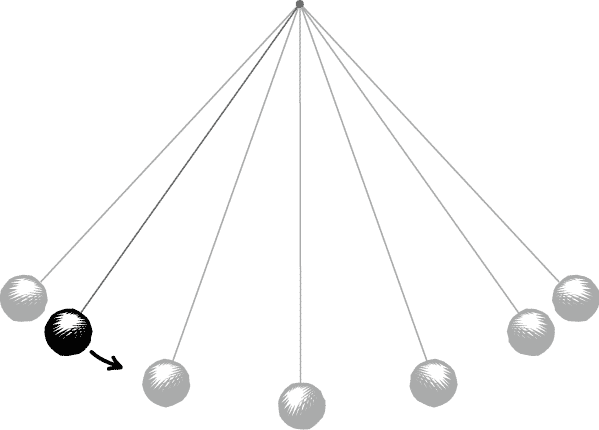
\includegraphics[width=0.6\linewidth]{Pictures/pendulum13}			
					\end{center}
				\end{column}	
				\begin{column}{.40\linewidth}
					\begin{center}
						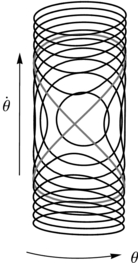
\includegraphics[width=0.45\linewidth]{Pictures/pendulum-phase-space}			
					\end{center}
				\end{column}	
			\end{columns}
			%
			\begin{defblock}[Symplectic Manifold]
				\vspace{-1em}
				\includestandalone[width=1\textwidth]{Pictures/Figure_sym}	
			\end{defblock}
			%
			\pause
			\begin{exblock}[$M = T^\ast Q$ is symplectic]
				with $\omega = d \theta $ given by
				$$ \left.\theta\right\vert_{(q,p)} (v) = p (\pi_\ast v) ~.$$
			\end{exblock}
			%
			\pause
			\vspace{1.2em}
			\centering
			\textit{ based on the notion of \\"states".}		
		\end{column}
		\onslide<1->{\vrule{}}
		\pause
		\begin{column}{.50\linewidth}
			\centering
			\textit{ "algebraic approach" to mechanics \dots}
			\vspace{.5em}	
			\begin{defblock}[Classical Observables]
				Unital, associative, commutative algebra $C^\infty(M)$.
			\end{defblock}
			%
			\vspace{.1em}
			\pause
			\begin{defblock}[Hamiltonian vector fields]
				$\vHam_f \in \mathfrak{X}(M)$ such that:
				$$\iota_{\vHam_f} \omega = -df \quad$$ %$\in B^1(M)$
				%
				\footnotetext{	$\vHam_f$ = \emph{Ham.v.f. pertaining to $f\in C^\infty(M)$}.}
			\end{defblock}
			\vspace{.1em}
			%
			\begin{defblock}[Poisson Algebra of Observables]
				$C^\infty(M)$ is a Poisson algebra with
				$$\{f,g\} = \iota_{\vHam_g} \iota_{\vHam_f} \omega = \omega(\vHam_f,\vHam_g) ~.$$
			\end{defblock}
			%
			\pause
			\vspace{.15em}
			\centering
			\textit{ based on the notion of \\"measurable quantities".}						
		\end{column}
	\end{columns}
\end{frame}
\note[itemize]{
		\footnotesize 
		\item We work in the framework of multisymplectic geometry which is one of the possible generalizations of the well-established field of symplectic geometry.
		\item To recall what symplectic geometry is let me assume a particular point of view: mechanics.
		\\
		Idea:"
		Symplectic geometry is a branch of differential geometry studying symplectic manifolds; it originated as a formalization of the mathematical apparatus of classical mechanics and geometric optics."{\href{https://ncatlab.org/nlab/show/symplectic+geometry}{nlab}}
		\\
		Namely, a sym. mfd. is the geometric structure encoding the phase space of conservative, autonomous, ordinary, classical, mechanical systems.
		\item 	{Geometrically: a Symplectic manifold $(M,\omega)$} $M$ a smooth manifold, $\omega\in \Omega^{2}(M)$ closed and non-degenerate, i.e. $d\omega=0$ and  $\omega^\flat:TM\to T^*M, v\mapsto \iota_v\omega$ is injective.
		\item
		Examples: orientable 2-manifolds with volume (e.g. $S^2$, $T^2$, $\mathbb R^2$), cotangent bunlde $T^*Q$ of any manifold $Q$ (with $\omega=d\theta$, $\theta_\eta(v)=\eta(T\pi_Q(v))$), coadjoint orbits. 
		\item $\theta$ = \emph{tautological 1-form}.
			$\theta$ evaluated at $p\in T^*Q$ in the fibre of $q\in Q$ and contracted with $v$ coincides with the form $p$ evaluated at $q$ and contracted with the push forward of $v$.
		\item We identify a special class of vector fields.
			Out of them one can define a Lie bracket.
		\item Poisson is a Lie algebra with the extra property of compatibility with the associative product (Leibniz rule)
		\item take away message: geometric (based on "states") vs algebraic (based on "measurable quantities").

}
%- . - . - . - . - . - . - . - . - . - . - . - . - . +

 




%-----------------------------------------------------------%
\subsection{Multisymplectic geometry}
%-----------------------------------------------------------%
 
%- . - . - . - . - . - . - . - . - . - . - . - . - . - . - . - . - . - . - . - . - . - . - . - .%
\begin{frame}{From symplectic to {multi}symplectic} 
	%
	\begin{center}
		$-$ \emph{multisymplectic means \textbf{going higher} in the degree of $\omega$} $-$
	\end{center}
	\pause
	\begin{defblock}[$n$-plectic manifold ~\emph{(Cantrijn, Ibort, De Le\'on)} \cite{Cantrun2017}]
		\includestandalone[width=0.95\textwidth]{Pictures/Figure_multisym}	
	\end{defblock}
	%
	\pause
		\begin{table}
			\begin{tabular}{c c c}
				symplectic forms \small($n=1$) & $\leftrightsquigarrow$ & volume forms \small($n= \text{dim}(M)-1$)
			\end{tabular}
		\end{table}

	\vfill
	\pause
	\begin{block}{Historical motivation}
		Mechanics: geometrical foundations of \textit{(first-order)} field theories.
	\end{block}
	%
	\begin{table}
		\ifHandout
		%
		\else
		\only<4>{
		\begin{tabular}{|p{0.2\textwidth}|p{0.3\textwidth}|p{0.35\textwidth}|} 
            \hline
            \parbox[][20pt][c]{0.2\textwidth}{mechanics} & \multicolumn{2}{c|}{geometry} \\
            \hline
            \parbox[][20pt][c]{0.2\textwidth}{phase space} & symplectic manifold &  \\[.25em]
            \parbox[][20pt][c]{0.2\textwidth}{classical \\ observables} & Poisson algebra &  \\[.25em]
            \parbox[][20pt][c]{0.2\textwidth}{symmetries} &  group actions admitting comoment map &  
            \\
            \hline
  \multicolumn{1}{c}{}
            &  \multicolumn{1}{@{}c@{}}{$\underbrace{\hspace*{.3\textwidth}}_{\text{point-like particles systems}}$} 
            &  \multicolumn{1}{@{}c@{}}{}              \\
		\end{tabular}
		}
		\fi
		\onslide<5->{
		\begin{tabular}{|p{0.2\textwidth}|p{0.3\textwidth}|p{0.35\textwidth}|} 
            \hline
            \parbox[][20pt][c]{0.2\textwidth}{mechanics} & \multicolumn{2}{c|}{geometry} \\
            \hline
            \parbox[][20pt][c]{0.2\textwidth}{phase space} & symplectic manifold & multisymplectic manifold \\[.25em]
            \parbox[][20pt][c]{0.2\textwidth}{classical \\ observables} & Poisson algebra & $L_\infty$-algebra \\[.25em]
            \parbox[][20pt][c]{0.2\textwidth}{symmetries} &  group actions admitting comoment map & group actions admitting (homotopy) comomentum map
            \\
            \hline
  			\multicolumn{1}{c}{}
            &  \multicolumn{1}{@{}c@{}}{$\underbrace{\hspace*{.3\textwidth}}_{\text{point-like particles systems}}$} 
            &
            \multicolumn{1}{@{}c@{}}{$\underbrace{\hspace*{.3\textwidth}}_{\text{field-theoretic systems}}$} 
               \\
		\end{tabular}
		}
	\end{table}	




\end{frame}
\note[itemize]{
	\item Historically, the interest in multisymplectic manifolds, has been motivated by the need for understanding the geometrical foundations of first-order classical field theories.
	The key point is that, just as one can associate a symplectic manifold to an ordinary classical mechanical system (e.g. a single
point-like particle constrained to some manifold), it is possible to associate a multisymplectic
manifold to any classical field system (e.g. a continuous medium like a filament or a fluid). See frame Extra-\ref{Frame:Ms-Field-Mechanics} 
	
	\item General ideas basic parallelisms with caveats
	\item caveat: points in multiphase spaces are not states
	\item the table hides the duality between geometric and algebraic approaches to the problem.
	\item	Mechanics: geometrical foundations of \textit{(first-order)} field theories.
		\begin{itemize}
		 \item[-] Kijowski, W. Tulczyjew \cite{Kijowski1979}; %(1979)
		 \item[-] Cariñena, Crampin, Ibort \cite{Carinena1991b};% (1991)
		 \item[-] Gotay, Isenberg, Marsden, Montgomery \cite{Gimmsy1};%(1998)
		 \\ $\cdots$
		\end{itemize}
	\item {Def. Multisymplectic manifold $(M,\omega)$}
	$M$ a smooth manifold, $\omega\in \Omega^{n+1}(M)$ closed and non-deg., i.e.: $d\omega=0$ and $\omega^\flat:TM\to \Lambda^nT^*M, v\mapsto \iota_v\omega$ is injective.
	\item Examples: orientable $n{+}1$-manifolds with volume (e.g. $S^{n+1}$, $T^{n+1}$, $\mathbb R^{n+1}$ ), multicotangent bunlde $\Lambda^nT^*Q$ of any manifold $Q$ (with $\omega=d\theta$. $\theta_\eta(v_1,...,v_n)=\eta(T\pi_Q(v_n),...,T\pi_Q(v_n))$),  semisimple Lie groups, hyperKähler manifolds,...
 	\item Without the non-deg. condition we call it \emph{premultisymplectic}. 

}
%- . - . - . - . - . - . - . - . - . - . - . - . - . - . - . - . - . - . - . - . - . - . - . - .%


%-----------------------------------------------------------%
\subsection{Higher Observables}
%-----------------------------------------------------------%

%- . - . - . - . - . - . - . - . - . - . - . - . - . - . - . - . - . - . - . - . - . - . - . - .%
\begin{frame}{Observables in $n$-plectic geometry}
	%
	\begin{defblock}[Hamiltonian $(n-1)$-forms]
		\begin{displaymath}
			\Omega^{n-1}_{ham}(M,\omega) 	:=
			\biggr\{ \sigma \in  \Omega^{n-1}(M) \; \biggr\vert \; 
				\exists \vHam_\sigma \in \mathfrak{X}(M) ~:~ 
				\tikz[baseline,remember picture]{\node[rounded corners,
                        fill=orange!5,draw=orange!30,anchor=base]            
            			(target) {$d \sigma = -\iota_{\vHam_\sigma} \omega$ };
            	}				
				~\biggr\} 
		\end{displaymath}
	\end{defblock}
%
%	\pause
%		\tikz[overlay,remember picture]
%		{
%			\node[rounded corners,
%                 fill=orange!5,draw=orange!30,anchor=base]
%            	 (base) at ($(current page.north east)-(2,1)$) [rotate=-0,text width=3.5cm,align=center] {\footnotesize{\textcolor{red}{Hamilton-DeDonder-Weyl \\equation}}};
%		}	
%	\begin{tikzpicture}[overlay,remember picture]
%    	\path[->] (base.south) edge[bend right,red](target.north);
%    \end{tikzpicture}
	%
	\vfill
	\begin{columns}[T]
		\pause
		\setlength{\belowdisplayskip}{5pt}
		\begin{column}{.50\linewidth}
			%
			\vspace{-1em}
			\begin{thmblock}[Observables $L_\infty$-algebra]
				$\Omega^{n-1}_{ham}(M,\omega)$ endowed with
				\vspace{-.5em}
				\begin{displaymath}
					\lbrace \sigma_1, \sigma_2 \rbrace =			
					~ - \iota_{\vHam_1}\iota_{\vHam_2} \omega 
				\end{displaymath}			
				can be "completed" to a \\ $L_\infty$-algebra.
			\end{thmblock}
			%	
		\end{column}	
		%
		\pause
		\begin{column}{.50\linewidth}
		%
			\begin{itemize}
				\item[\cmark] Skew-symmetric;
				\item[\xmark] multiplication of observables;
				\item[\xmark] Jacobi equation;
				%\\ \hspace*{4.25em} full-fledged Jacobi equation;
				\item[\smark] Jacobi equation \emph{up to homotopies}.
			\end{itemize}			
			%
				\[
					\small
					\{\alpha,\{\beta,\gamma\}\} + \text{\it cyc. perm.}
					= {\color{orange}\d \iota_{X_\alpha} \iota_{X_\beta} \iota_{X_\gamma}\omega}
				\]
		\end{column}	
	\end{columns}
	%
	\vfill
	\pause
	Interesting alternatives:
	\begin{itemize}
		\item  descend to $\Omega^{n-1}_{ham}(M) / {\color{orange}\d\hspace{1pt}\Omega^{n-2}(M)}$, hence getting a Lie algebra;
		\item Incorporate the {\color{orange}discrepancy} as part of the data of the space of observables 
				$L_\infty(M,\omega) = \Omega_{ham}^{n-1}(M)\oplus{\color{orange}\Omega^{\leq n-2}(M)}$.
			%a \textbf{homotopy Lie algebra} or \textbf{$L_\infty$-algebra}.
	\end{itemize}
	
	
\end{frame}
\note[itemize]{
	\item In the paper 
 \href{https://www.sciencedirect.com/science/article/pii/S0393044018301189}{Invitation to Multisymplectic Geometry} \cite{RYVKIN20199}\	, the equation highlighted in orange, which defines Hamiltonian forms, is referred to as the Hamilton--DeDonder--Weyl equation---a somewhat imaginative extension compared to its traditional formulation in \href{https://en.wikipedia.org/wiki/De_Donder\%E2\%80\%93Weyl_theory}{De Donder--Weyl theory}. 
	\item a **Hamiltonian $(k-1)$-form** $\alpha \in \Omega^{k-1}(M)$ is one that admits a vector field $X$ (a *Hamiltonian field*) satisfying $i_X\omega = d\alpha$. We call the pair $(X,\alpha)$ a *Hamiltonian pair*. 
	\item Just as in the symplectic case $(k=1)$ where $\alpha$ is a 0-form (function) and $X$ its Hamiltonian vector field, here $\alpha$ plays the role of the observable (often called an $(k-1)$-form observable). 
	\item The collection of all such Hamiltonian forms (for various degrees) can be organized into a graded object, and Rogers showed that it carries a canonical **$L_\infty$-algebra structure** .
    \item  **Example:** For a 3-plectic manifold (degree 3 form $\omega$), one has Hamiltonian 1-forms: each 1-form $\alpha$ for which there exists $X$ with $i_X\omega = d\alpha$. These Hamiltonian pairs $(X,\alpha)$ form the degree-0 part of the observables. In addition, ordinary functions (0-forms) can be viewed as Hamiltonian 0-forms (with $X$ such that $i_X\omega = d(0) = 0$), and perhaps higher-degree observables appear up to degree 1 in this case. The resulting $L_\infty$ has non-trivial brackets of arity up to 2 (making it a *Lie 2-algebra* of observables, a kind of higher Poisson algebra). The 2-bracket extends the Poisson bracket, and a 3-bracket arises measuring the failure of the Jacobi identity (something that vanishes in the symplectic case but not in general). For a 4-plectic form, one would get a Lie 3-algebra, etc.
}
%- . - . - . - . - . - . - . - . - . - . - . - . - . - . - . - . - . - . - . - . - . - . - . - .%



%- . - . - . - . - . - . - . - . - . - . - . - . - . - . - . - . - . - . - . - . - . - . - . - .%
\begin{frame}[fragile,t]{$L_\infty$-algebra of Observables (higher observables) }
	Let be $(M,\omega)$ a $n$-plectic manifold.
	\begin{defblock}[$L_\infty$-algebra of observables ~\emph{(Rogers)} ~\cite{Rogers2010}]
		
		\hspace{.25em} $L\infty(M,\omega)$ is given by:
		
		\begin{itemize}
			\item[•] a cochain-complex $(L,\{\cdot\}_1)$ 
		\end{itemize}
		\begin{center}
		\ifHandout
			\includestandalone{Pictures/Figure_Observables}	
		\else
			\includestandalone{Pictures/Frame_Observables}
		\fi				
		\end{center}
		\onslide<2->{
			\begin{itemize}
				\item[•] with $n$ (skew-symmetric) multibrackets $(2 \leq k \leq n+1)$
			\end{itemize}
			\begin{center}
				\includestandalone{Pictures/Equation_Multibracket}	
			\end{center}
		}
		%
	\end{defblock}
  \end{frame}
 \note[itemize]{
	\item if symplectic manifolds are the symmetric take on mechanics, Poisson algebras are the algebraic counterpart.
 	\item A Lie algebra is associated to an ordinary symplectic manifold (its Poisson algebra).
	%(Underlying this is a Lie algebra, whose Lie bracket is the Poisson bracket.)
	Similarly, one associates an Lie-$n$ algebra to any $n$-plectic manifold.
 	% https://ncatlab.org/nlab/show/n-plectic+geometry 	 
 	 %https://ncatlab.org/nlab/show/Poisson+bracket+Lie+n-algebra
	 \item Basically, the higher observables algebra is a chunk of the de Rham complex of $M$ with inverted grading( convention employed here) and an extra structure called "multibrackets".
 	\item ( In the 1-plectic case it reduces to the corresponding Poisson algebra of classical observables)
 	\item Rogers associated to any n-plectic mfd a $L\-\infty$ algebra, Zambon generalized it to the pre-n-plectic case.
 	\item Recognize in the definition of $\{\cdot,\ldots,\cdot\}_k$ the contraction with hamiltonian fields $v_\sigma$ w.r.t. $\sigma$.
  	\item Note $	\iota_{v_{\sigma_1}}\cdots\iota_{v_{\sigma_k}} = (-)^{(k-1)+(k-2)+\dots+1}\iota_{v_{\sigma_k}}\cdots\iota_{v_{\sigma_1}} = (-)^{\frac{k(k-1)}{2}}\iota_{v_{\sigma_k}}\cdots\iota_{v_{\sigma_1}}$ 
 	The definition usually find in literature of Rogers multibrackets involves the coefficient $ (-)^{\frac{k(k-1)}{2}} = -\varsigma(k-1) = (-)^{k+1} \varsigma(k)$.
  \item higher observables is Special instance of a more general object  called $L\-\infty$ Algebra...
 }
%- . - . - . - . - . - . - . - . - . - . - . - . - . - . - . - . - . - . - . - . - . - . - . - .%


 

%-----------------------------------------------------------%
%------------------------------------------------------------------------------------------------
\begin{frame}{Reminder: $L_\infty$ Algebras}

		\emph{
			$L_\infty$-algebra is the notion that one obtains from a Lie algebra when one requires the Jacobi identity to be satisfied only up to a higher coherent chain homotopy.
		}
		\\
		\vspace{.5em}
		\begin{defblock}[$L_\infty$-algebra ~\emph{(Lada, Markl, Stasheff)} ~\cite{Lada1993}\cite{Lada1995}]
			\includestandalone{Pictures/Figure_Linfinitydef}
		\end{defblock}	
		%
		%
	\pause
 

	\begin{itemize}
		\item<2-> You can construct a coalgebra out of $L$ \\
			{\small \color{UniGreen} (the reduced cofree coalgebra $S^{\geq 1}(L[1]),\Delta)$)}.
		\item<3-> You can assemble all $\mu_k$ to get a coderivation $Q_\mu$\\
				{\small \color{UniGreen} (the unique lift to a coderivation of the decalage of $ \mu=	\mu_1+\mu_2 + \dots$) }.
		\item<4-> Higher Jacobi is tantamount to having $Q_\mu ^2 = 0$.
	\end{itemize}
\end{frame}
\note[itemize]{
	\item $L_\infty$-algebra is the notion obtained from a Lie algebra requiring that the Jacobi identity is satisfied only up to a higher coherent chain homotopy.
	\item The Lie-n algebra mentioned before is a $L_\infty$ algebra with underlying graded vector space concentrated in degrees $0,1...n$.
	
	\item Definition. We say that a permutation $\sigma \in S_n$ is a $(j,n-j)$-unshuffle, $0\leq j \le1 n$  if $\sigma(1)< \dots < \sigma(j)$ and $\sigma(j+1)<\dots<\sigma(n)$.
	\\
	You can also say that $\sigma$ is a $(j,n-j)$-unshuffle if $\sigma(i)< \sigma(i+1)$ when $i\neq j$.

	\item 	Alternatively, the Jacobiators can be also denoted as $$\displaystyle J_m=\sum_{i+j=m+1} 	\mu_i \triangleleft \mu_j = 0$$
	employing the so-called \emph{ Richardson-Nijenhuis product}
		 $$\mu_i\circ \mu_j := (-)^{i(j+1)}\frac{1}{j!(i-1)!}\mu_i \triangleleft \mu_j\otimes \mathbb{1}_{i-1} \circ \mathcal{A}~,$$
		 where $\mathcal{A}$ denotes the (graded) total skew-symmetrizator.
		 
	\item see frame extra-\ref{Frame:unwapping-Jacobi} for a slightly demystification of the higher Jacobi equations.

	\item more precisely this statement is a proposition/definition

}
%------------------------------------------------------------------------------------------------


%%-----------------------------------------------------------%
%-----------------------------------------------------------%
\subsection{Goals}
%-----------------------------------------------------------%

%-----------------------------------------------------------%
\begin{frame}[fragile]{Scope / Goals}
	\begin{upshotblocktitle}
		\begin{itemize}
			\item[$\bullet$] Observables $L_\infty$-algebra construction is purely algebraic!
			\begin{itemize}
				\item[$\cdot$] \emph{(It relies only on the \underline{standard Cartan calculus identities} for differential forms and vector fields.)}
			\end{itemize}\pause
			\item[$\bullet$] Possible generalization to \underline{BV-modules over a Gerstenhaber algebra!}
			\begin{itemize}
				\item[$\cdot$] \emph{(A suitably general framework to formalize Cartan calculus.)}
			\end{itemize}
		\end{itemize}
	\end{upshotblocktitle}
	\pause \vfill

	\begin{claimblocktitle}
		To any given BV-module over a Gerstenhaber algebra together with a chosen closed element (a "cocycle") in the module, we can define:
		\begin{itemize}
			\item[$\cdot$] Hamiltonian pairs,
			\item[$\cdot$] together with an associated $L_\infty$-algebra structure.
		\end{itemize}
	\end{claimblocktitle}
	\pause \vfill

	\begin{outlookblock}[Applications]
		A more conceptual picture for the algebraic reduction of the observables $L_\infty$-algebra in presence of constraints / symmetries.
	\end{outlookblock}
	\vfill

\end{frame}
\note[itemize]{
	\item   Cartan's identities ensure that the operations $d, i_X, L_X$ behave in a coordinated way (the essence of *Gerstenhaber algebra and BV-module* structure, as we formalize below). 
	\item Rogers’ $L_\infty$ brackets are built using these ingredients: e.g., the binary bracket of two Hamiltonian forms $(X,\alpha)$ and $(Y,\beta)$ can be defined as $( [X,Y],; L_X\beta)$ (or plus cyclic terms), and higher brackets involve expressions with $i_{X_i} i_{X_j}\omega$ contracted with another argument, etc., ensuring the homotopy Jacobi identities hold .
	\item The key point is that all such formulas **only use the algebraic operations $d,i,L,[\cdot,\cdot]$ and the form $\omega$**. This algebraic nature allows generalization to any context where similar operators exist.
	\item *Limitations of Classical Reduction:** Before moving to the algebraic setup, note that reducing multisymplectic systems geometrically (analogue of Marsden-Weinstein reduction) can be challenging. Classical symplectic reduction requires a Lie group action that is free and proper and a regular value of the moment map; these conditions often fail (especially in field theory or higher form cases). Recent work has approached reduction **algebraically** by focusing on the algebra of observables (functions/forms) with constraints, rather than the quotient of manifolds. This algebraic approach, implemented for multisymplectic manifolds in Blacker-Miti-Ryvkin 2024, allows handling singular cases (non-free actions, etc.) by *encoding constraints and symmetries at the algebraic level.
Our work builds on this idea using *constraint triples*.
\item Given any Gerstenhaber algebra $G$ together with a BV-module $M$ and a chosen closed element (a  "cocycle ") $c$ in $M$, we will show how to construct an associated $L_\infty$-algebra of observables without reference to any underlying manifold .
\item Moreover, we will address how to perform reduction of these observables $L_\infty$-algebras in the presence of constraints or symmetries. For this, we employ the notion of constraint triples as an algebraic framework for coisotropic reduction. Adapting this to our BV-module setting, we obtain a general procedure to reduce an $L_\infty$ of observables, even in singular scenarios where classical quotient constructions fail  
}
%-----------------------------------------------------------%	

 


%-----------------------------------------------------------%
\ifstandalone
% https://en.wikibooks.org/wiki/LaTeX/Bibliographies_with_biblatex_and_biber
\begin{frame}[t,allowframebreaks]{Bibliography}
	%\nocite{*}
	\printbibliography
\end{frame}
\fi
%-----------------------------------------------------------%


%-----------------------------------------------------------+
\end{document}
%-----------------------------------------------------------+


